\chapter{THE PACKET PIPELINE PROCESSING MODEL} \label{ch:pipeline_model}

The Flowpath runtime environment uses an abstract switch model depicted in Figure \ref{fg:abstract_switch}. The switch model is composed of three major components: the Steve application, ports, and a controller. This chapter is dedicated to describing these components.

\begin{figure}[ht]
\includegraphics[width=\textwidth]{switch}
\caption{The abstract switch model is composed of three major components: the Steve application, ports, and an internal controller.}
\label{fg:abstract_switch} 
\end{figure}

Steve applications are executable, dynamic link libraries which are loaded by the Flowpath runtime environment. Steve is distinct from other SDN languages in that it compiles into modules which implement parts of \textit{both} the data and control planes. 

Steve \textit{pipelines} are part of the data plane which forwards packets. Packets are sent and received on ports which reside on the data plane. As Flowpath receives packets, it sends them through the Steve application's pipeline. This pipeline is an algorithm that determines where a packet is forwarded. The Steve pipeline is discussed in the following Section \ref{pipeline_desc}.

Steve \textit{event handlers} are part of the control plane. Part of the responsibility of the control plane is to augment the forwarding behavior of the data plane when necessary. Event handlers are executed when some exceptional event has arisen and the behavior of the pipeline must change. Event handling and the Flowpath controller are discussed later in Section \ref{events_desc}.

\section{The Steve Pipeline} \label{pipeline_desc}

Steve uses an abstract model known as \textit{pipeline processing} to process packets. Steve pipeline processing model can be described in terms of four phases: 1)
\textit{ingress processing}, 2) \textit{decoding stages}, 3) \textit{table
matching stages}, and 4) \textit{egress processing}. Figure
\ref{fg:pipeline_model} depicts this pipeline processing model.

\begin{figure} [ht] \includegraphics[width=\textwidth]{pipeline}

\caption{The flow of a packet through the Steve pipeline. The first phase is
ingress processing, where a \textit{context} (described in Section
\ref{context_desc}) is built around the packet. Decoding stages decode and
extract. Tables match packets and perform actions. Event processing may take
place on special circumstances Egress processing decides where a packet is
forwarded (or dropped).} \label{fg:pipeline_model} 
\end{figure}

Describing these phases will be the topic if this chapter. One must understand this model to be able to write a Steve pipeline application.

The Steve \textit{pipeline} is a subset of the processing model depicted in Figure \ref{fg:pipeline_model}. A pipeline is a composition of decoding stages and table matching stages. These stages are known as \textit{pipeline stages}. Each stage is connected to the next in such a way that the output of
one stage becomes the input to the next. Pipeline stages may be connected in a number of flexible ways. This the the topic of Section \ref{pipeline_comp_desc}. 

The pipeline processing model is essentially a
state machine. Each pipeline stage is a state in the machine. Each state has a
set of conditions which, when met, causes the packet to move to new stages, or
new states. This can be represented as a graph where each pipeline stage is a
node on the graph and each stage is connected to the next with an edge. The graph representation allows the Steve programming language to analyze these
pipelines using graph algorithms to confirm certain safety guarantees.

The Steve programming language allows programmers to express
\textit{decoding} and \textit{table matching} stages.
Steve pipeline programs follow a run-to-complete model of execution. Once a
packet enters the pipeline, each stage is consecutively applied to
the packet. Once no more stages are applied, the packet exits the pipeline and
the next packet enters.

\section{Ingress Processing} \label{ingress_desc}

A packet enters a network device on a port, known as its \textit{ingress port}.
At this time, the data plane builds a data structure known as the
\textit{context} around the packet. This context is what the pipeline uses to
save data as the packet moves between pipeline stages. Further explanation of the
context can be found in Section \ref{context_desc}.

After ingress processing, the data plane dispatches the context (which includes
the packet) to the first decoding stage. The ingress processing stage is not
something that is written in a Steve application. It is implicit and handled by
the Flowpath runtime discussed in Chapter \ref{ch:flowpath}.

\subsection{Packet Context} \label{context_desc}

Pipeline stages are connected in such a way that the output from one stage
becomes the input to the next. The \textit{context} data structure is that
output and input. It carries data between stages. A stage often needs to use
data created by prior stages. As a packet moves between stages, information such
as the position and length of extracted fields and headers must be saved for
later recovery. Specifically, a Steve context saves the following data:

\begin{itemize} \item The packet itself. From now on, anytime mention of the
context is made, it is implied that this also includes the packet itself. \item
The packet's logical and physical ingress ports. \item The egress port. This
field is written to during pipeline processing. It ultimately determines which
port the packet gets forwarded on. \item The packet's length. \item A tunnel
identifier. \item The offset and length of decoded fields saved in a
\textit{binding environments}. \item The offset of decoded headers saved in a
\textit{binding environment}. \item An action set that may be written to and is
executed during egress processing. \end{itemize}

Extracted fields and headers get saved in \textit{binding environments}
contained within the context. The term \textit{environment} refers to a data
structure which maps names (in this case field and header names) to their
storage location during runtime \cite{compilers1}. The mapping of those storage
locations to the values held there is known as \textbf{state}. There is a
binding environment for fields and headers respectively.

Figure \ref{fg:ContextEnv} depicts the binding environment. The field binding
environment is used to map fields to  \{\textit{offset},\textit{length}\} pairs, where \textit{offset} is the absolute offset of the beginning of the field from the beginning of the packet (in bytes) and \textit{length} is the length of the field (in bytes). The header binding environment similarly maps headers to their absolute offset from the beginning of the packet. These mappings are known as \textit{bindings}.

\begin{figure} 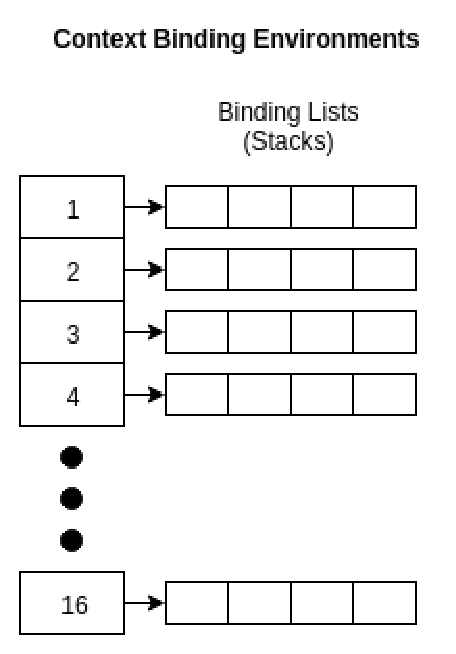
\includegraphics[scale=0.75,natwidth=203,natheight=298]{context}
\caption{The binding environment inside a context used to store the length and
offset of fields, or the offset of headers. On the left, indexes one through
sixteen represent the fields that can be extracted. Each field maintains a
binding stack. Each element in the binding stack is a binding which stores the
offset and length where an instance of that field can be found. }
\label{fg:ContextEnv} \end{figure}

Since any given packet can contain one or more of any field or header with the
same name, a binding environment maintains a stack for every field and header.
These stacks are called \textit{binding stacks}. By extension, this means an
environment is actually a mapping of field names to binding stacks. When the
value of a field is needed, the topmost binding on the binding stack, i.e. the most recently extracted field with that name, shall be
used to recover the value of that field.

Figure \ref{fg:ContextEnvWorking} demonstrates how data is stored in the context
as it is being decoded. The example is a packet which contains an encapsulated
IPv4 header commonly used in IP tunneling. First, the ethernet \texttt{macdst}
(mapped to index 0), \texttt{macsrc} (mapped to index 1), and \texttt{ethtype}
(mapped to index 2) fields are extracted and stored in the context. Then the
first IPv4 header's \texttt{ipdst} (mapped to index 3) and \texttt{iptype}
(mapped to index 4) fields are extracted. After that, another IPv4 header's
\texttt{ipdst} fields are extracted. If the value of
\texttt{ipdst} is used in the program, it is the second one which gets used.

\begin{figure}[ht]
\begin{subfigure}[t]{.45\textwidth}
  \centering
  \includegraphics[width=.8\linewidth]{cxt_pkt_ex}
  \caption{An example packet with ethernet, IPv4, and nested IPv4 header.}
  \label{fg:view1}
\end{subfigure}%
\hfill
\begin{subfigure}[t]{.45\textwidth}
  \centering
  \includegraphics[width=.8\linewidth]{cxt_s1}
  \caption{Binding the fields in the ethernet header.}
  \label{fg:view2}
\end{subfigure}

\begin{subfigure}[t]{.45\textwidth}
  \centering
  \includegraphics[width=.8\linewidth]{cxt_s2}
  \caption{Binding fields from the first IPv4 header.}
  \label{fg:view3}
\end{subfigure}%
\hfill
\begin{subfigure}[t]{.45\textwidth}
  \centering
  \includegraphics[width=.8\linewidth]{cxt_s3}
  \caption{Binding fields from the second IPv4 header.}
  \label{fg:view4}
\end{subfigure}
\caption{A context environment in
action during runtime.} \label{fg:ContextEnvWorking} 
\end{figure}

The \textit{action set} is the other major data structure contained within the
context. An action set in Steve is a sequence of \textit{actions}. Actions are written to the action set for \textit{deferred execution}
through the course of pipeline processing. These actions are executed in the order with which they were written once the
packet completes pipeline processing, during the egress processing phase.

\section{Decoding Stage} \label{decoder_desc}

When a packet is received on its ingress port, it is a chunk of raw,
uninterpreted data. Before a packet can be processed and routed, its
fields must be decoded (found) and extracted (have their value recovered) so that meaningful decisions can be made
based on those values. Decoding stage, or \textit{decoders} for short, are
responsible for this.

Steve allows for programmers to specify \textit{how} and \textit{which} fields
are decoded. Decoded fields get saved in the context as \{\textit{offset},\textit{length}\} pairs, a
format inspired by POF \cite{pof, pof_fis, pof_impl}. The Steve compiler takes
care of generating these \{\textit{offset},\textit{length}\} pairs, lifting the error-prone burden
from the programmer. When the value of that field is required, the bytes are
extracted from the packet using these \{\textit{offset},\textit{length}\} pairs.

In some packet processing languages like P4 \cite{p4_spec, p4_spec2}, all
relevant headers have all their fields decoded from start to finish. All fields
are extracted and saved before any pipeline processing happens. This is what is
considered a \textit{full decode}. After this full decode, the decision making
process on the packet begins using those saved fields. However, this method is
inherently inefficient. Only certain fields and headers within a packet are ever
really needed. To compound this, different devices may care about different
subsets of fields within a given packet. Decoding all headers and fields from a
packet is inherently wasteful.

Full decodes waste valuable processing time. Efficiency is important when trying
to achieve data processing rates comparable to line rate (10Gbps to 40 Gbps). This inherent
inefficiency is why Steve proposes the idea of a \textit{partial decode}. Like
POF \cite{pof, pof_fis, pof_impl}, Steve is designed to allow programmers to
specify the extraction of only specific fields rather than an entire header.
Though the specification may be verbose in some cases, it makes programmers
think very carefully about which fields they need and which fields they do not.

Additionally, Steve proposes that not all headers need to be decoded. For
example, if a networking application only needs to forward using MAC addresses,
there is no reason to waste time extracting fields from IPv4 or IPv6 headers,
and so on. It is up to the programmer to express how deep they wish to look into a packet.

That being said, Steve also supports the full decode. It may be desirable to
some programmers to do this in certain scenarios, thus the language does not
favor one paradigm over another.

\section{Table Stage} \label{table_desc}

Table stages classify packets into groups based on values found in a subset of
that packet's extracted fields. In fact, it is a decision table, like those
found in heuristics applications. This is done through a mechanism known as a
flow table defined by the OpenFlow standard \cite{openflow_spec}. A sample flow table is depicted in Table \ref{tbl:flow_table}.

\begin{table}[ht]
\caption{An example flow table matches on IPv4 destination and TCP protocol destination port.}
\label{tbl:flow_table}
\centering
\begin{tabularx}{\linewidth}{| c | X | X | X |}
\hline
% Header of table
\multirow{2}{*}{Priority} & Key: IP Destination & Key: TCP Destination port  & \multirow{2}{*}{Actions} \\
\cline{2-3}
  & \multicolumn{2}{|c|}{Match Fields} & \\
\hline
\hline
% beginning of flows.
1 & 10.1.1.0 & 80 & Set IP Dest. equal to 192.168.1.30. Output to port 1. \\
\hline
1 & 192.168.1.31 & 23 & Drop packet. \\
\hline
1 & 192.168.1.32 & 443 & Output port 2. \\
\hline
... & ... & ... & ... \\
\hline
\end{tabularx}
\end{table}


A \textit{flow table} has a \textit{key} and a set of \textit{flow entries}. A
key specifies a set of fields, called \textit{key fields}, that a table matches
against (or classifies with). They are the equivalent of decision attributes.

Table \ref{tbl:flow_table} has two key fields: IP destination and TCP destination port. A table is said to \textit{match on} its key fields.

A flow entry is equivalent to a rule in a decision table. Each flow entry is
composed of \textit{match fields}, a \textit{priority}, a set of
\textit{actions}, and miscellaneous additional metadata (called
\textit{properties}). Table \ref{tbl:flow_table} has three sample flow entries. 

For each key field, each flow entry has a corresponding value, known as a
\textit{match field}, such that every flow entry in the table is uniquely
identified by its match fields and its priority. When a packet is being matched
against a table, the fields given by the table's key are extracted from the
context. These extracted fields, together, are called the \textit{query key}.
Each match field is then compared against the corresponding packet field. If all
fields match, then the flow entry's actions are executed on the packet. Actions
may modify the packet, context, or flow tables. Priority is used to
unambiguously execute exactly one flow entry if multiple flow entry matches are
found. The highest priority flow entry is always executed.

For example, if a packet with an IP destination of 10.10.1.0 and a TCP port destination of 80 were matched against Table \ref{tbl:flow_table}, it would match the first flow entry. It would have its IP destination changed to 192.168.1.30, then it would be forwarded to port 1.

If no flow entry matches the packet's field values, the \textit{miss case} flow
entry is applied to the packet instead. By default, a miss case will drop the
packet, but the behavior can be user defined. Miss cases always have the lowest
possible priority amongst flow entries and each match field can be considered a
wildcard.

The mechanic of table matching is also analogous to that of relational or SQL
tables (which coincidentally can be used to implement decision tables). In fact,
Frenetic, another packet processing language, uses SQL-inspired syntax to
classify packets \cite{foster2011frenetic, foster2013frenetic}. If we make this
comparison, a flow table is analogous to a relational table, the concept of a
key is the same for both, and a flow entry is analogous to a tuple in a SQL
table. Each packet and its fields "queries" the table for flow entries with
matching keys.

\section{Egress Processing} \label{egress_desc}

Pipeline processing completes when a pipeline stage has finished executing
without sending the packet to a new stage. At this point the packet exists the
pipeline and enters egress processing.

First, all actions written the context action set are executed. Then the data
plane will check the egress port field in the context. If this has been set,
then the data plane will queue the packet up to be forwarded through that port.
Otherwise, the packet is dropped. The context is then destroyed.

\section{Actions} \label{action_desc}

Actions may modify a packet, forward it, move it to a new stage, or modify a
flow table. This section summarizes the current actions supported by Steve.
These actions may be applied during any processing stage.

\begin{itemize}

\item \textbf{Output.} The output action will forward a copy of a packet to a given
port. If this action is written to the action set, when executed during egress
processing, it writes the given port to the context's egress port field which
determines where that packet gets forwarded.

\item \textbf{Drop.} The drop action drops a packet.

\item \textbf{Decode and goto.} These actions are known as \textit{transition
actions}. They end the current stage and send the context to a new stage. The
decode action sends the context to a given decoder. Goto sends the context to a
given flow table.

\item \textbf{Raise.} Raise sends a copy of the context and an event handler to be
executed by the controller port. The original packet continues through pipeline
processing as usual.

\item \textbf{Insert and remove flow entry.} These actions can insert or remove a flow
entry with given match fields. Inserting a flow entry that already exists will
eject the old one and replace it with the new one. Removing a non-existent flow
entry does nothing.

\item \textbf{Set.} The set action will overwrite the bytes in a field with a given
value.

\item \textbf{Write.} Write action allows actions to be written to the context's
action set. Only set and output actions may be written.

\item \textbf{Clear.} The clear action removes all actions from the action set.

\end{itemize}

\section{The Flowpath Controller and Event Handling} \label{events_desc}

Once pipeline processing is completed by the Steve application, the packet is forwarded on a port. Occasionally, the Steve pipeline will choose to forward to a special port called the \textit{controller port}. The controller port is connected to a Flowpath thread of execution known as a \textit{controller}. A controller executes functions, known as \textit{event handlers}, which deal with exceptional events. The controller queues these packets and executes Steve event handlers on them. This mechanic is known as the \textit{event stage}.

An event stage is not part of the typical pipeline processing model.
Event stages execute when the Steve programmer decides that special
circumstances have arisen, and some packet processing should happen outside the
run-to-completion pipeline processing model. Certain slower operations which can
bottleneck the run-to-completion pipeline are typically performed in event
stages. This usually involves inserting or removing flow entries from flow
tables when unexpected packets have been found.

The Steve programmer defines a set of event handler functions. An event handler
takes a copy of the context and performs some set of operations with it. An
event stage executes when the programmer sends a copy of the context and an
event handler to a controller using the raise action summarized in Section
\ref{action_desc}.

The Flowpath runtime does not use the same external controller mechanic as other SDN switches, namely OpenFlow \cite{openflow_spec}. To reduce the latency of sending messages to an external controller, Flowpath is capable of executing Steve-defined event handlers internally.

\section{Pipeline Composition} \label{pipeline_comp_desc}

Kinds of processing stages can be interleaved together in any order within the
pipeline. This means that Steve is capable of supporting different packet
processing paradigms found in other research such as POF \cite{pof, pof_fis,
pof_impl} and P4 \cite{p4_spec, p4_spec2}. With the Steve pipeline specification
language a user can specify that a pipeline does:

\begin{enumerate} \item \textbf{A full decode of the packet followed by a
sequence of tables.} Packets have all necessary headers and fields decoded and
saved in the context first. The packet is then dispatched to the first table in
the pipeline. From there, matched flow entries dictate which table the packet is
sent to next or which port the packet is forwarded to.

\item \textbf{A chain of partial decodes and table lookups.} Packets get
partially decoded and dispatched to a table. The flow entry could carry the
packet to another table, another decoder, or forward it out of the network. The
pipeline is thus a chain of alternating sequences of decoding stages and table
matching stages. \item \textbf{Only decodes.} In some special cases, it may not
even be necessary to go to a table matching stage. It may be possible to make a
decision about the packet’s ultimate destination immediately upon evaluating a
certain field within the packet using a simple conditional statement
(if-statement, if-else statement, etc). Therefore, decoding stages also support
the range of actions supported by flow entries, which can include outputting
packets to a port or dropping it. \end{enumerate}

Upon entering the pipeline, a packet must first go through at least one decoding
stage before moving to the next processing stage. From there, the packet
transitions from one stage of the pipeline to the next. With each stage, certain
conditions are evaluated which will determine where the packet must flow next.
Finally, the packet will exit the pipeline either through a port(s) or by being
dropped and discarded.

